\section{Data Collection Performance}
\label{sec-performance}

In this section we assess the performance of the {\em Fetch} data collection
protocol. We evaluate Fetch in terms of its {\em yield}, its ability 
to successfully collect requested data; and its {\em latency}, the 
time to download events from the network.

\subsection{Data yield}

We define the {\em event yield} of a Fetch transfer as the fraction of
nodes for which the entire 60~sec signal was successfully downloaded
following an event. The calculation only considers those nodes that
were active at the time of the event detection (Figure~\ref{fig-nodesalive}). 
For example, if 10~nodes were active
during an event, then the event yield is defined in terms of 10~nodes.
Note that the Fetch protocol attempts to download a signal from all
active nodes, even those that did not detect the event.

\begin{figure}[t]
\begin{center}
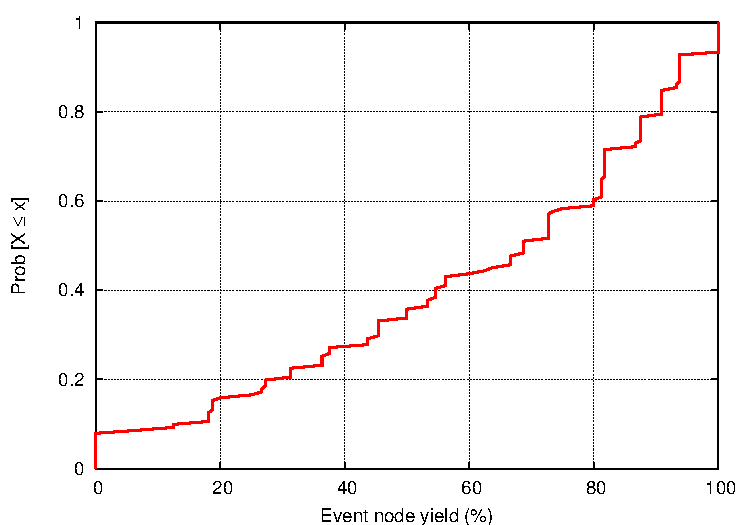
\includegraphics[width=\hsize]{./evaluation/figs/performance/yields/comparison/availableEventNodeYieldCDF.pdf}
\end{center}
\caption{\small{\bf Event yield.}
{\em This graph shows a CDF of the event yield for each of the 229~events
recorded during the entire deployment. Event yield is the fraction of
active nodes from which a complete 60~sec signal was downloaded
following an event.}}
\label{fig-compBlockYieldCDF}
\end{figure}

Figure~\ref{fig-compBlockYieldCDF} shows a CDF of the event 
yield for all 229~events recorded during the deployment.  As the
figure shows, the median event yield was 68.5\% and the 90th
percentile was 94\%.  The yield can be affected by several factors.
First, the protocol will abort a transfer from a node after
re-requesting the same block more than 20~times, or if the transfer
from a single node exceeds 10~minutes.  Second, because sampling is
disabled while performing a data transfer, if two back-to-back events
occur a node may not end up storing data for the second event.


% ------ Original text ------------------------
%% In this section we assess the performance of the {\em Fetch} data collection
%% protocol. We evaluate Fetch in terms of its {\em yield}, its ability 
%% to successfully collect requested data; and its {\em latency}, the 
%% time it took to download events from the network.

%% \subsection{Data yield}
%% %  - Yield [KL]
%% %    - % of detected events that we successfully downloaded data for
%% %    - How much data per event
%% %    - Consider all nodes vs. only "active" nodes
%% %    - Before and after reprogram

%% We define the {\em event block yield} of a Fetch transfer as the fraction of
%% requested data blocks successfully downloaded from each node following an
%% event. The calculation only considers those nodes that were operational at
%% the time of the event detection. For example, if 10~nodes were active during an
%% event, then the event block yield is defined as the fraction of data blocks
%% retrieved from those 10~nodes.  Normally, following an event the system would
%% attempt to download 60~sec of data from each operational node, including
%% nodes that did not report the event. 

%% \begin{figure}[t]
%% \begin{center}
%% 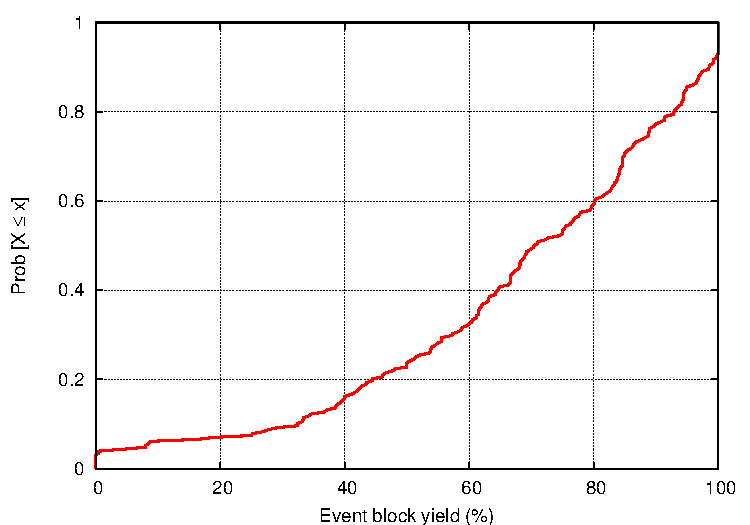
\includegraphics[width=\hsize]{./evaluation/figs/performance/yields/comparison/schBlockYieldCDF_entire.pdf}
%% \end{center}
%% \caption{\small{\bf Event block yield.}
%% {\em This graph shows a CDF of the event block yield for each of the 229~events
%% recorded during the entire deployment.}}
%% \label{fig-compBlockYieldCDF}
%% \end{figure}

%% Figure~\ref{fig-compBlockYieldCDF} shows a CDF of the event block
%% yield for all 229~events recorded during the deployment.  As the
%% figure shows, the median event block yield was 70.4\% and the 90th
%% percentile was 98.6\%.  The yield can be affected by several factors.
%% First, the protocol will abort a transfer from a node after
%% re-requesting the same block more than 20~times, or if the transfer
%% from a single node exceeds 10~minutes.  Second, because sampling is
%% disabled while performing a data transfer, if two back-to-back events
%% occur a node may not end up storing data for the second event.
% --------------------------------------------------------


%The event block yield of each transfer is affected by several factors.
%First, the Fetch protocol will timeout on a transfer from a node after
%re-requesting the same block more than 20~times, or if the cumulative
%transfer time from a single node exceeds 10~minutes.	Second, the protocol
%may request blocks not in a node's cache.  Because we disable sampling during
%a Fetch transfer, if two back-to-back events occur the second Fetch operation
%may attempt to request blocks that the node never stored because it was busy
%with the first transfer. Or we may simply fail to disable sampling on a
%particular node causing the requested blocks to be overwritten before we are
%able to retrieve them. 

%Also shown is a breakdown of the
%event block yield both before and after the network was reprogrammed on
%August 11, 2005 following the Deluge failure. After the
%reprogramming, the median event block yield improved from 66.7\% to 77.8\%. 

%The improvement is due to several changes that were introduced
%following the reprogramming in an attempt to improve the performance
%and robustness of the Fetch protocol based on our observations in the
%first few days of the deployment.  First, the transfer timeout was
%increased from 10~minutes to 20~minutes, giving nodes more time to
%respond to Fetch requests. Second, the speed at which Fetch commands
%were propagated through the network was increased by a factor of~4,
%decreasing the latency for a Fetch request to reach a node.  Third, we
%disabled duplicate suppression in the flooding protocol used to
%propagate Fetch requests to the network, increasing overall network
%load but increasing reliability.

%Figure~\ref{fig-compNodePercentiles} shows the 50th-percentile yield
%for each node before and after network reprogramming.  The yield for
%most nodes is very good (100\% in most cases), with a couple of
%exceptions.  In general, the yield is highest for nodes that were
%closest to the root of the tree and for those that only had 2
%channels.  This is consistent with our expectations.  When the base
%station concludes that there was an event, it first floods the network
%with a command telling nodes to stop sampling.  Afterwards, it
%downloads the event data from each node in a round-robin fashion,
%ordered by hop count from the root.  We observed that the stop
%sampling message did not always propagate to all the nodes, with nodes
%farter away from the root beeing less likely to have received the stop
%sampling command.  If a node did not stop sampling, there was a good
%chance that it might have overwritten it's circular flash buffer by
%the time it was scheduled to be downloaded.  Again this is more likely
%for nodes farter away because they were scheduled later.  The two
%nodes with 4 channeles, 250 and 251, produce twice as much data than
%the 2-channel nodes and therefore fill in their falsh at twice the
%rate.  Note that node 251 was also the second farthes node from the
%root after node 214.
%
%In Figure~\ref{fig-compNodePercentiles} we also see that after the
%network reprogramming, the yield for each node improved or stayed the
%same.  \XXXnote{add explanations}.

%\begin{figure}[t]
%\begin{center}
%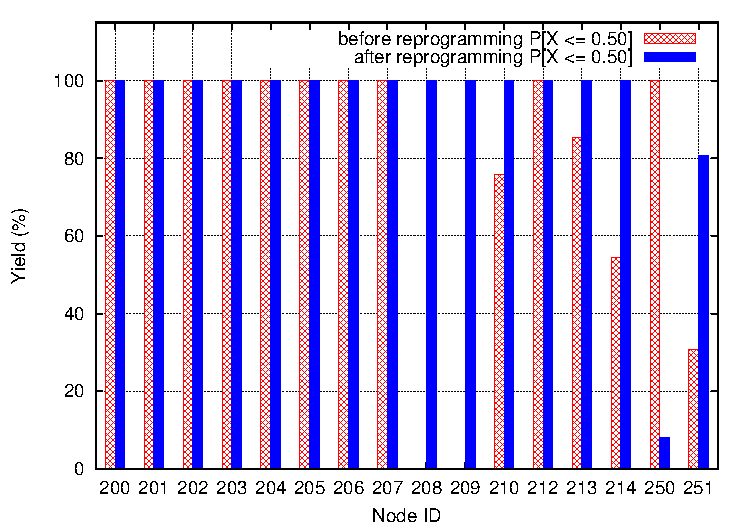
\includegraphics[width=\hsize]{./evaluation/figs/performance/yields/comparison/nodePercentiles.pdf}
%\end{center}
%\caption{\small{\bf 50th-percentile yield by nodeID before and after network reprogramming.}
%{\em The 50th-percentile yield for most of the nodes is very good,
%with a few exceptions.  After the network reprogramming, the yield for
%all nodes either improved or stayed the same.}}
%\label{fig-compNodePercentiles}
%\end{figure}

%% \XXXnote{MDW: The previous definition of ``node yield'' did not make
%% sense to me. I have tried to reword this but Konrad needs to check
%% that this is right. It does not make sense to ``download a node.''}

Next, we look at the {\em node yield} which we define as the
probability that an event was successfully downloaded from a given
node.  Like the event yield, the calculation only considers those
nodes that were active at the time of each event detection.  Node yield
can be affected by several factors.  The depth and radio link quality
of a node's routing path to the base station affect packet loss rate
and thereby the likelihood of a Fetch timeout.
%The farther a node
%is from the root of the tree, 
%and the more low-quality links it has to route
%across, 
%the more likely its packets will get lost.  
Additionally, two nodes outfitted with triaxial seismometers
(nodes~250~and~251) sample and store twice as much data as the others,
increasing the probability of a timeout.  Finally, a bug in our control
application caused node~250 to sample data continuously, even during a Fetch
operation. As a result, this node was more likely to overwrite an 
event stored in flash before it could be downloaded.

\begin{figure}[t]
\begin{center}
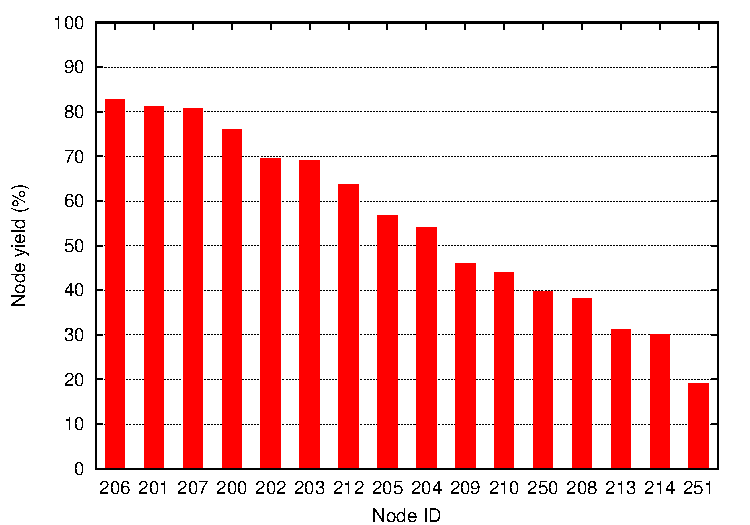
\includegraphics[width=\hsize]{./evaluation/figs/performance/yields/nodeYield/nodeYieldOnly.pdf}
\end{center}
\caption{\small{\bf Node yield.}
{\em This graph shows the node yield for each of the 16 nodes
over the entire deployment, defined as the probability that an event
was successfully downloaded from a node, as long as that node is active 
during the corresponding event detection.}}
\label{fig-nodeYield}
\end{figure}

%% \XXXnote{MDW: I am very confused by this figure and the terminology
%% here. What does ``the total number of times a node was available and
%% successfully downloaded'' mean? I think we should probably just
%% eliminate the extra bars from the figure here, and only show the node
%% yield by itself. We have already shown the node uptimes in another figure.}

Figure~\ref{fig-nodeYield} shows the node yield for each of the nodes.
%% For comparison, it also shows the total number of times a node was
%% available and successfully downloaded for the entire deployment.  
We can see how the factors mentioned above affected performance.
First, the nodes with the highest yield (above 80\%) tend to be within
two hops from the root (see Figure~\ref{fig-schematic}).  However,
despite being within two or three hops, node~209 had a fairly low
yield.  This is explained by the fact that node~209 had a poor link to
its closest parent, node~200.  In fact, although most nodes had a
stable parent throughout the deployment, node~209 used node~200 as its
parent only 33\% of the time and nodes 206~and~207 the remaining 66\%
of the time.  Node~213 also switched parents between nodes
204~and~208, but unlike node~209 it was always three hops away.
Node~214 was the farthest node in terms of hopcount and as a result
had one of the lowest yields.  The larger amount of data was also a
factor for the four-channel nodes, 250~and~251. In addition, node~251
was five radio hops from the gateway.


% -------- Original text ---------------------------------------------
%% Next, we look at the {\em node block yield} which we define as the fraction
%% of requested data blocks successfully downloaded from each node.
%% The node block yield can be affected by several 
%% factors. The depth and radio link quality of a node's routing path 
%% to the base station affect packet loss rate and thereby the likelihood
%% of a Fetch timeout.
%% %The farther a node
%% %is from the root of the tree, 
%% %and the more low-quality links it has to route
%% %across, 
%% %the more likely its packets will get lost.  
%% Additionally, two nodes outfitted with triaxial seismometers
%% (nodes~250~and~251) sample and store twice as much data as the others,
%% increasing the likelihood of failure.  Finally, a bug in our control
%% application caused node 250 to sample data continuously, even during a Fetch
%% operation. As a result, this node was more likely to overwrite an 
%% event stored in flash before it could be downloaded.

%% \begin{figure}[t]
%% \begin{center}
%% 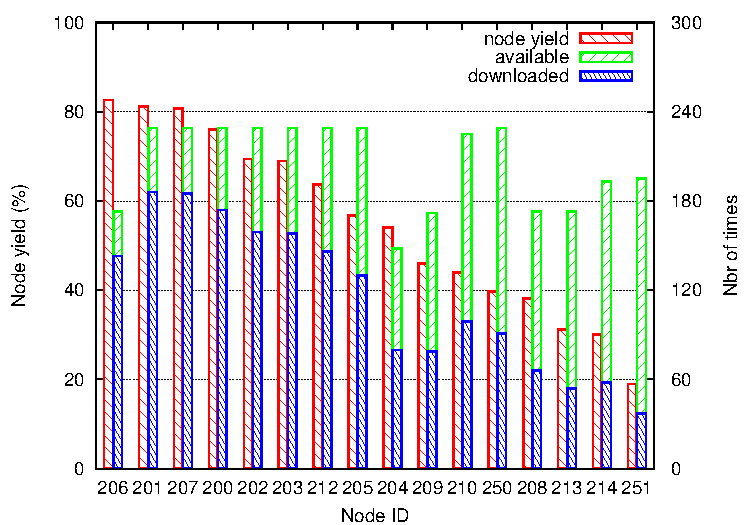
\includegraphics[width=\hsize]{./evaluation/figs/performance/yields/nodeYield/nodeYield.pdf}
%% \end{center}
%% \caption{\small{\bf Node block yield.}
%% {\em This graph shows the node block yield for each of the 16 nodes
%%   over the entire deployment. For comparison, the graph also shows the
%% total number of scheduled and downloaded blocks for each node on the 
%% right-hand $y$-axis.}}
%% \label{fig-nodeYield}
%% \end{figure}

%% Figure~\ref{fig-nodeYield} shows the node block yield for each of the nodes.
%% For comparison, it also shows the total number of blocks scheduled and
%% downloaded for the entire deployment.  We can see how the factors mentioned
%% above affected performance.  First, the blocks with the highest yield (above
%% 85\%) tend to be within two hops from the root (see
%% Figure~\ref{fig-schematic}).  However, despite being within two or three hops
%% node~209 had one of the lowest yields.  This is explained by the fact that
%% node~209 had a poor link to its closest parent, node~200.  In fact, although
%% most nodes had a stable parent throughout the deployment, node~209 used 
%% node~200 as its parent only 33\% of the time and nodes 206~and~207 
%% the remaining 66\% of the time.  
%% Node~213 also switched parents between nodes 204~and~208, but
%% unlike node~209 it was always three hops away.  Node~214 was the farthest
%% node in terms of hopcount and as a result had one of the lowest yields.  
%% The larger amount of data was also a factor for the four-channel nodes, 
%% 250~and~251. In addition, node~251 was five radio hops from the gateway.
% --------------------------------------------------------------


%% ; node 250 was continousely sampling, and therefore Fetch could not %
%always reach it before it overwrote the relevant data.

%% \begin{figure}[t]
%% \begin{center}
%% 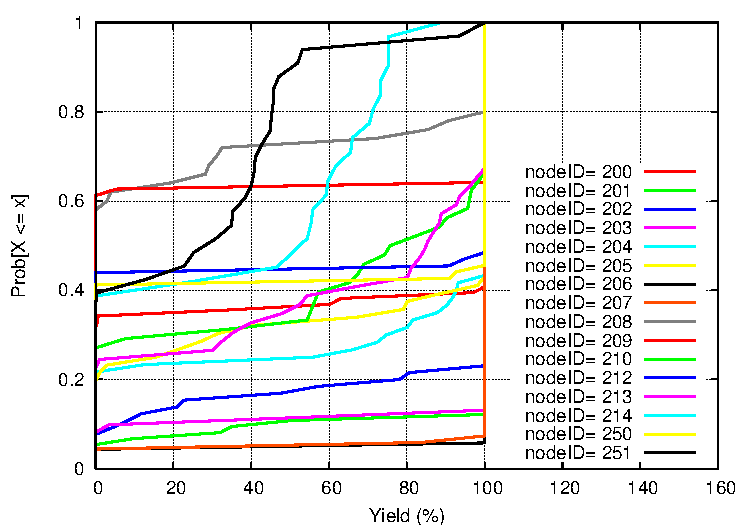
\includegraphics[width=\hsize]{./evaluation/figs/performance/yields/beforeReprogram/schBlockYieldCDFByNode.pdf}
%% \end{center}
%% \caption{\small{\bf Block yield by nodeID before network reprogramming.}
%% {\em This graph shows CDFs of the block yields for each node.  The
%% yields for some of the nodes is much higher (mostly the ones that were
%% farther in the routing tree) than for others.}}
%% \label{fig-blockYieldByNodeBeforeReprog}
%% \end{figure}

%% \begin{figure}[t]
%% \begin{center}
%% 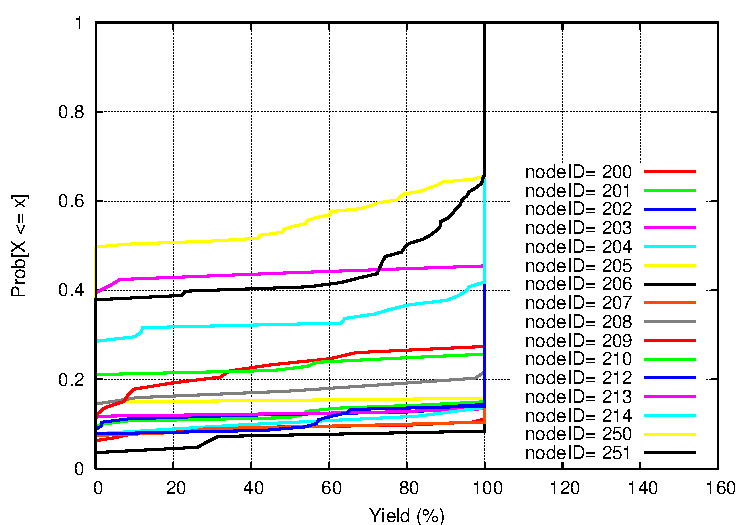
\includegraphics[width=\hsize]{./evaluation/figs/performance/yields/afterReprogram/schBlockYieldCDFByNode.pdf}
%% \end{center}
%% \caption{\small{\bf Block yield by nodeID after network reprogramming.}
%% {\em This graph shows CDFs of the block yields for each node.  The
%% yields for some of the nodes is much higher (mostly the ones that were
%% farther in the routing tree) than for others.}}
%% \label{fig-blockYieldByNodeAfterReprog}
%% \end{figure}


%% \begin{figure}[t]
%% \begin{center}
%% 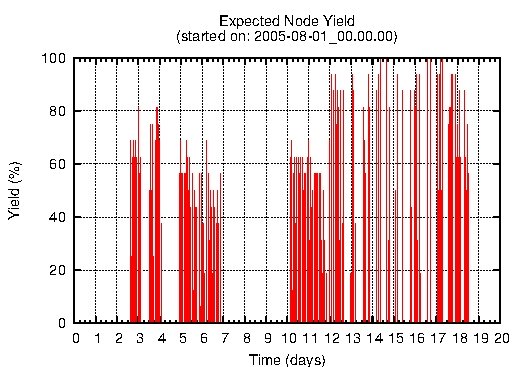
\includegraphics[width=\hsize]{./evaluation/figs/performance/yields/expNodeYield.pdf}
%% \end{center}
%% \caption{\small{\bf Expected node yield.}
%% {\em This graph shows the node yield out of the 16 nodes.  Only nodes
%% for which the enitre event was downloaded successfully are considered.}}
%% \label{fig-expNodeYield}
%% \end{figure}

%% \begin{figure}[t]
%% \begin{center}
%% 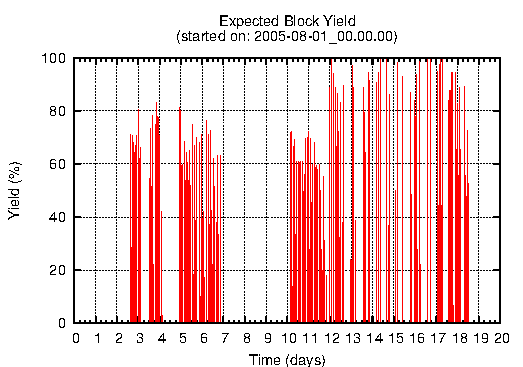
\includegraphics[width=\hsize]{./evaluation/figs/performance/yields/expBlockYield.pdf}
%% \end{center}
%% \caption{\small{\bf Expected block yield.}
%% {\em This graph shows the block yield out of the 16 nodes.  Only block
%% for which the enitre block was downloaded successfully are considered.}}
%% \label{fig-expBlockYield}
%% \end{figure}

%% \begin{figure}[t]
%% \begin{center}
%% 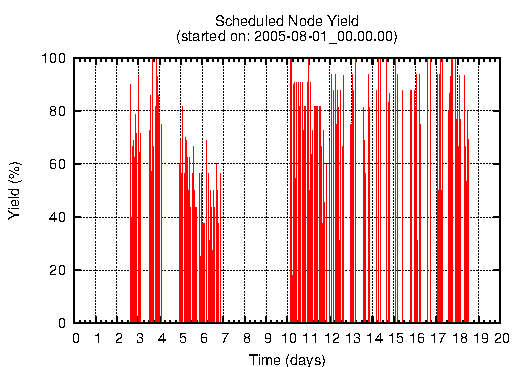
\includegraphics[width=\hsize]{./evaluation/figs/performance/yields/schNodeYield.pdf}
%% \end{center}
%% \caption{\small{\bf Scheduled node yield.}
%% {\em This graph shows the node yield out of the scheduled nodes for
%% each event.}}
%% \label{fig-schNodeYield}
%% \end{figure}

%% \begin{figure}[t]
%% \begin{center}
%% 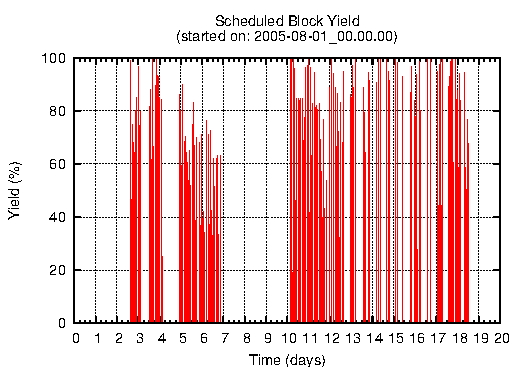
\includegraphics[width=\hsize]{./evaluation/figs/performance/yields/schBlockYield.pdf}
%% \end{center}
%% \caption{\small{\bf Scheduled block yield.}
%% {\em This graph shows the block yield out of the scheduled block for
%% each event.}}
%% \label{fig-schBlockYield}
%% \end{figure}

\subsection{Fetch latency}

Transfer latency directly impacts data yield. Because we disabled sampling on
each node (apart from node~250) during a Fetch download cycle, 
the duration of the data transfer also affects a node's ability to 
record back-to-back events.  

\begin{figure}[t]
\begin{center}
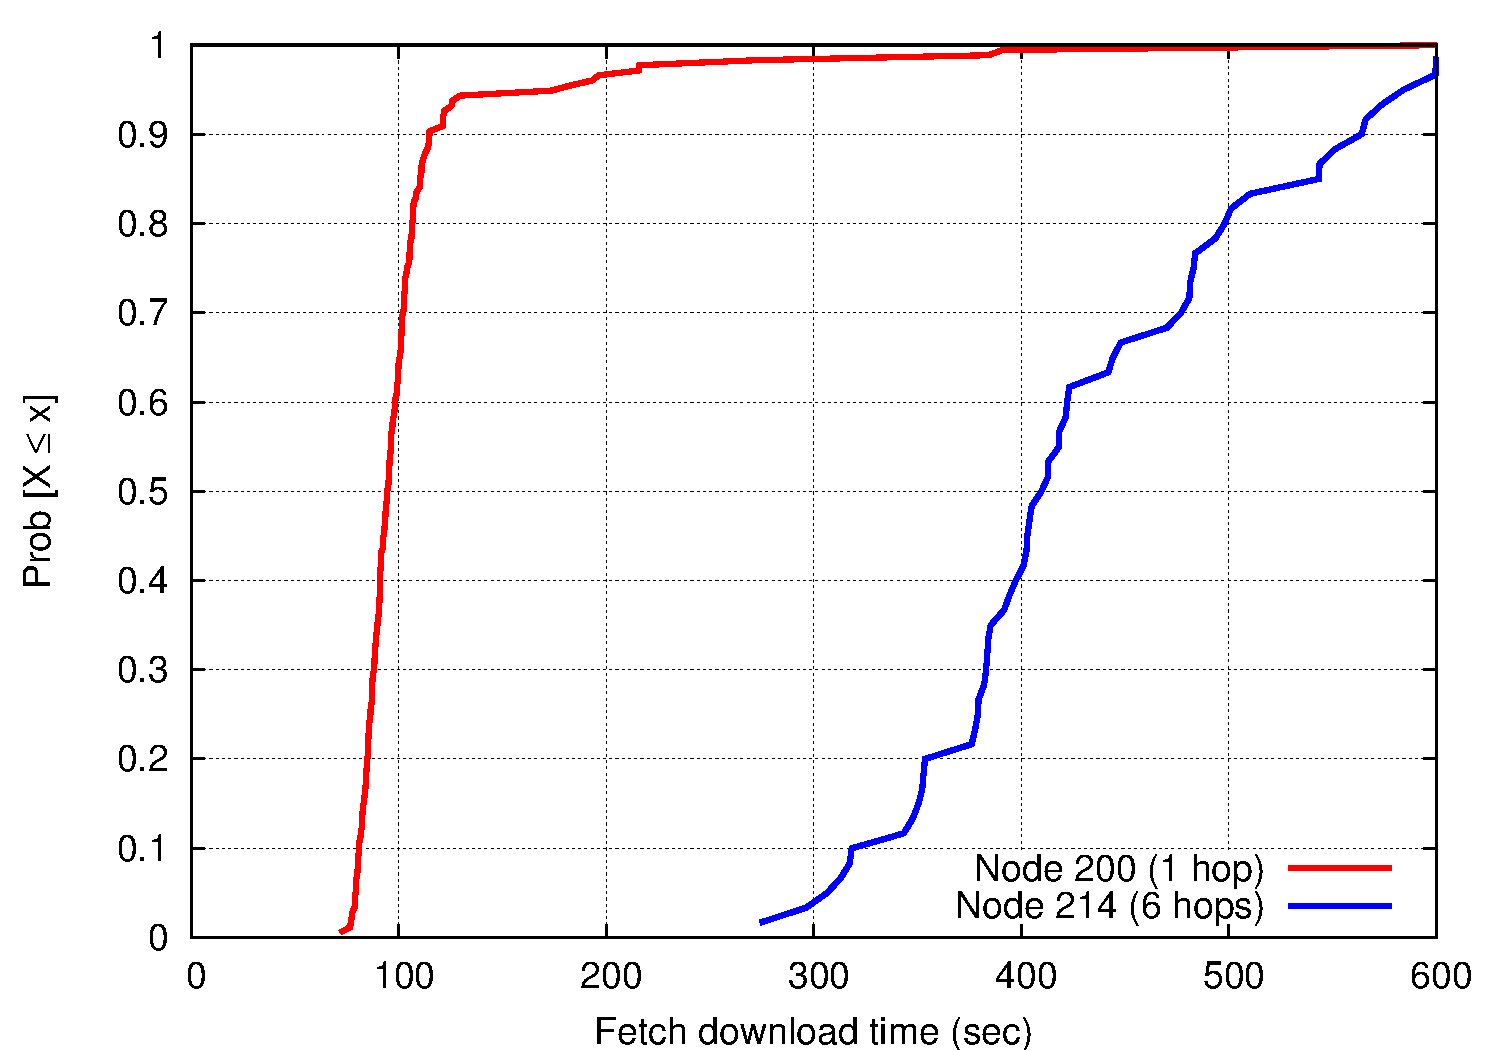
\includegraphics[width=\hsize]{./evaluation/figs/performance/CDFByHops/CDFBYHOPS.pdf}
\end{center}
\caption{\small{\bf Distribution of Fetch latency for two nodes.} {\em The
latency for a Fetch download depends on the depth of the node in the
routing tree, which affects both command propagation latency and
reliability of the routing path. Node~200 is located 1~hop from the 
sink and node~214 is located 6~hops away.}}
\label{fig-fetchlatency-byhops}
\end{figure}

The median latency for Fetch operations (downloading 60~sec worth of
data from a single node) was 186~sec and the 90th
percentile was 444~sec. Unsurprisingly, latency varies with the depth of
the node in the routing tree.  Figure~\ref{fig-fetchlatency-byhops}
compares Fetch latency for nodes 200~and~214, located 1~and~6 hops
away from the sink, respectively. Node~200 had a median Fetch latency
of 94~sec, while node 214~had a median latency of 409~sec,
about 63~sec per hop.  This is due to both increased delay for propagating
Fetch command messages, as well as increasing packet loss and
retransmission overheads as the data flows over multiple hops to the
base.

% 23 Apr 2006 : GWA : Need to discuss this in text... TODO.

%\begin{figure}[t]
%\begin{center}
%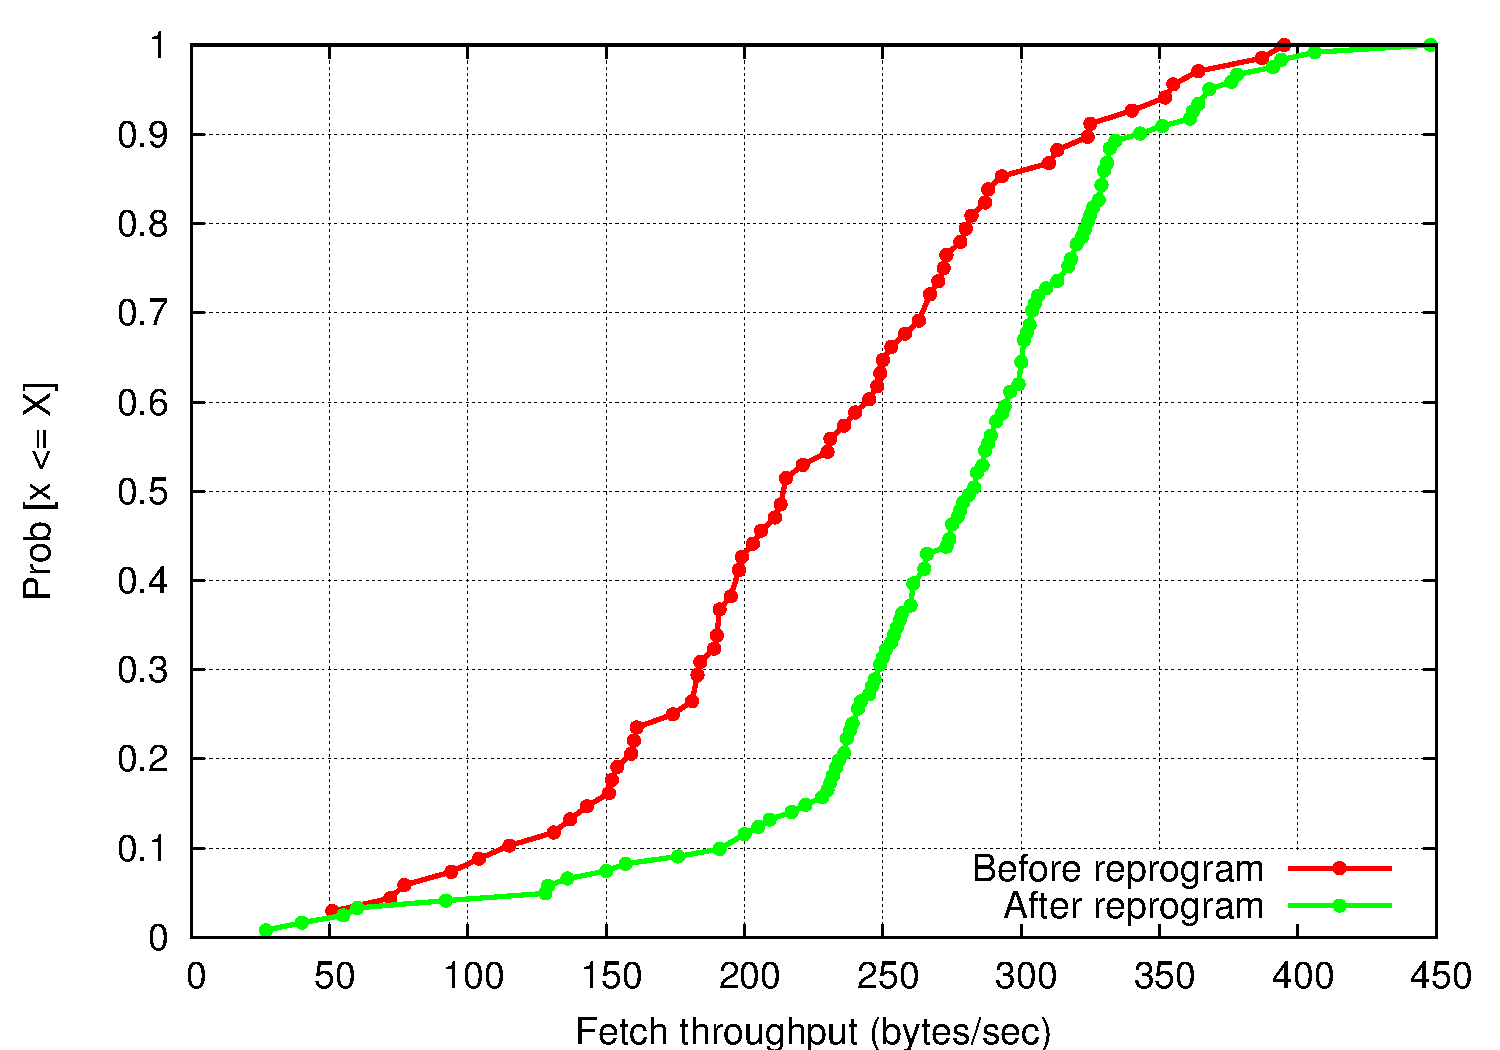
\includegraphics[width=\hsize]{./evaluation/figs/performance/fetchspeed/fetchspeed-cdf-oldnew.pdf}
%\end{center}
%\caption{\small{\bf Fetch throughput.}
%{\em This graph shows a CDF of the the throughput for each Fetch
%operation before and after the node reprogram. 
%Before programming, the median throughput was XXX~bytes/sec and after
%the median was~XXX~bytes/sec.}}
%\label{fig-fetchspeed-oldnew}
%\end{figure}

%Figure~\ref{fig-fetchspeed-oldnew} shows a CDF of the throughput of
%each Fetch operation from each node following an event. Before
%the network reprogram on August 11, the median throughput was
%215~bytes/sec; after the reprogram the median increased to 283~bytes/sec.
%While these values are far less than the peak thoughput achievable
%by the radio (which can exceed 12000 bytes/sec when MAC delays
%are accounted for), it is important to note that the Fetch protocol
%was never designed to maximize throughput. In particular, the 
%protocol requests a single block at a time from the network, and
%uses a long delay (up to 1~sec) before retransmitting a block request.

Fetch was initially designed to support reliable downloads of infrequent
events and we did not anticipate the need to capture back-to-back signals.
Unfortunately, these were common at Reventador, and may necessitate a
redesign. For example, it may be possible to reduce latency by streaming
multiple blocks in one request and reconstructing partial blocks after a
burst. Caching recently-received blocks on intermediate nodes could reduce
latency for repair requests~\cite{netshm-emnets05}.  However, such changes
would greatly increase the complexity of the protocol. For this deployment
we opted to prioritize simplicity and stability over performance.

%   - Throughput by hopcount
%\begin{figure}[t]
%\begin{center}
%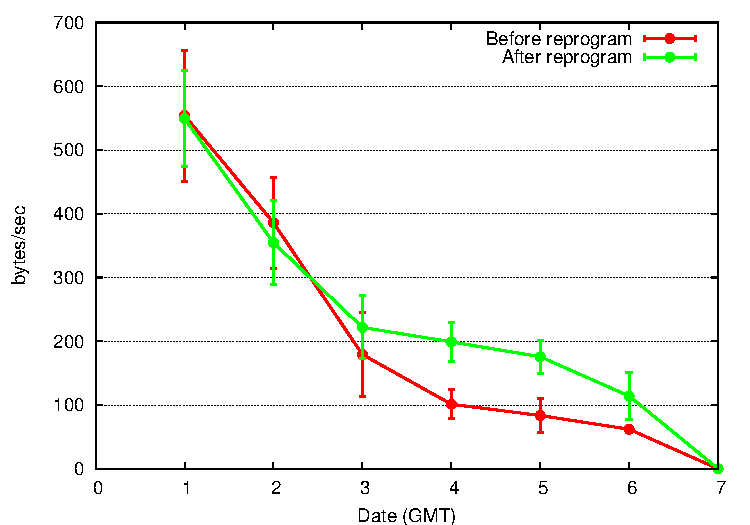
\includegraphics[width=\hsize]{./evaluation/figs/performance/fetchspeed-byhops/fetchspeed-oldnew.pdf}
%\end{center}
%\caption{\small{\bf Fetch throughput by node hop count.}
%{\em The throughput of fetch downloads diminishes rapidly as the
%hopcount distance to the node increases. This is due to increased
%packet loss and longer latencies for propagating fetch command
%messages. After reprogramming, fetch throughput increases primarily
%for nodes several hops from the base station.}}
%\label{fig-fetchspeed-byhops}
%\end{figure}

%  - Throughput [MDW]
%    - Bytes/sec
%\begin{figure}[t]
%\begin{center}
%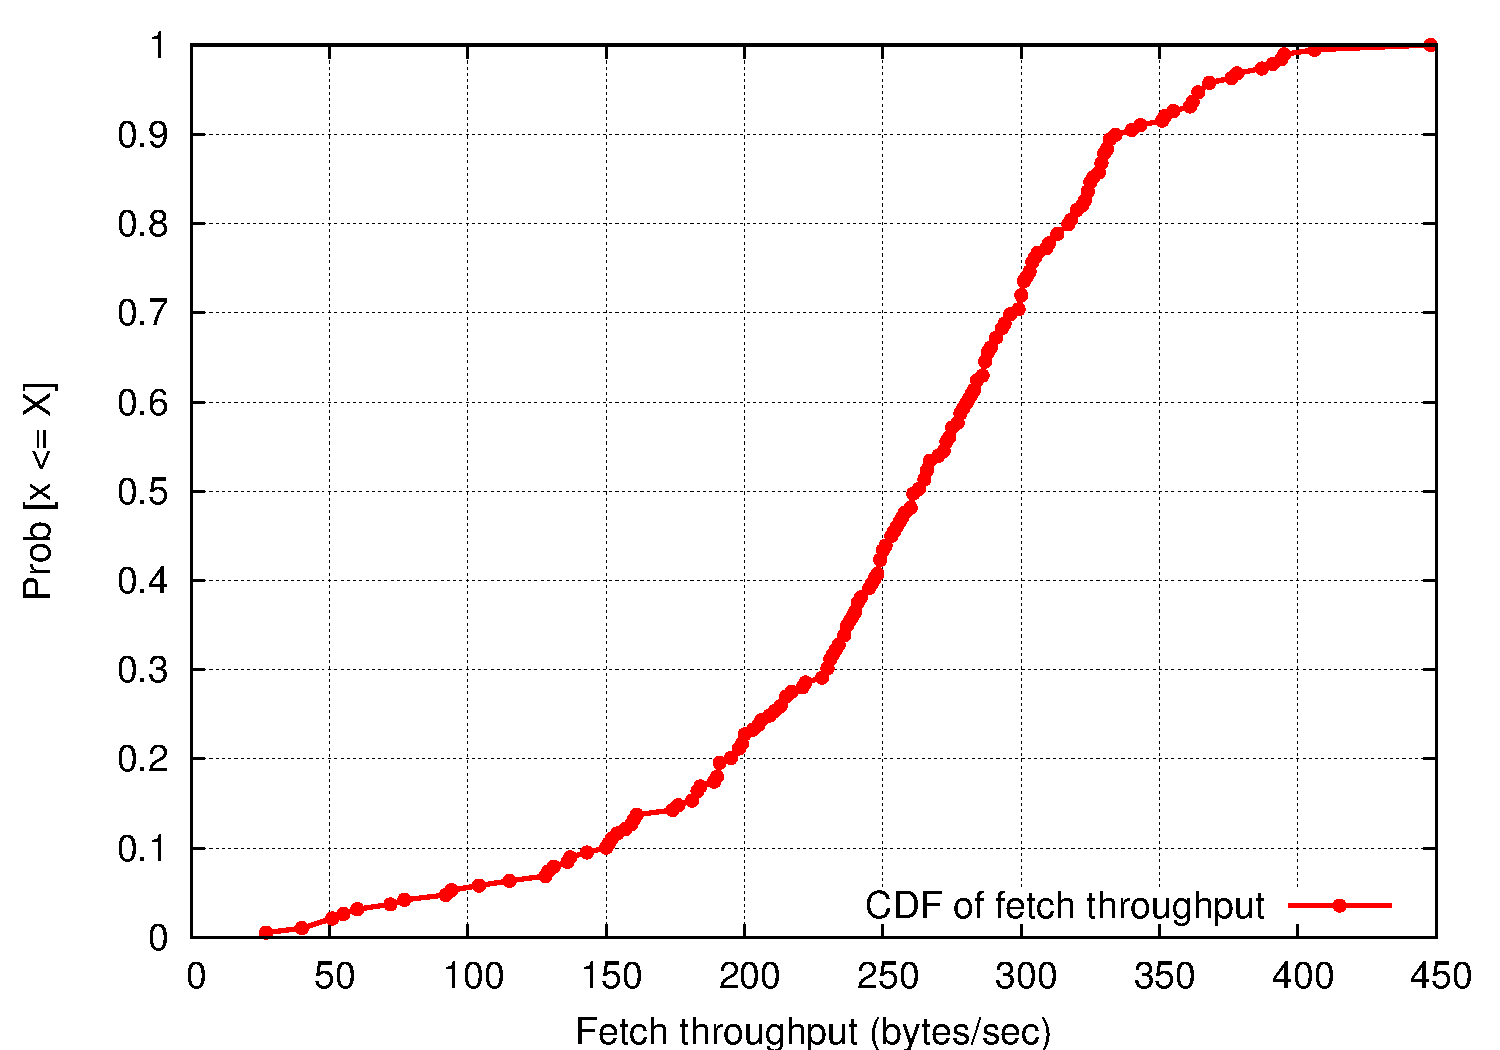
\includegraphics[width=\hsize]{./evaluation/figs/performance/fetchspeed/fetchspeed-cdf.pdf}
%\end{center}
%\caption{\small{\bf Fetch throughput.}
%{\em This graph shows a CDF of the the throughput for each fetch
%operation. The median throughput was XXX~bytes/sec and the
%mean~XXX~bytes/sec.}}
%\label{fig-fetchspeed}
%\end{figure}

% 23 Apr 2006 : GWA : Need to discuss this in text... TODO.

%    - Latency for data transfer
%\begin{figure}[t]
%\begin{center}
%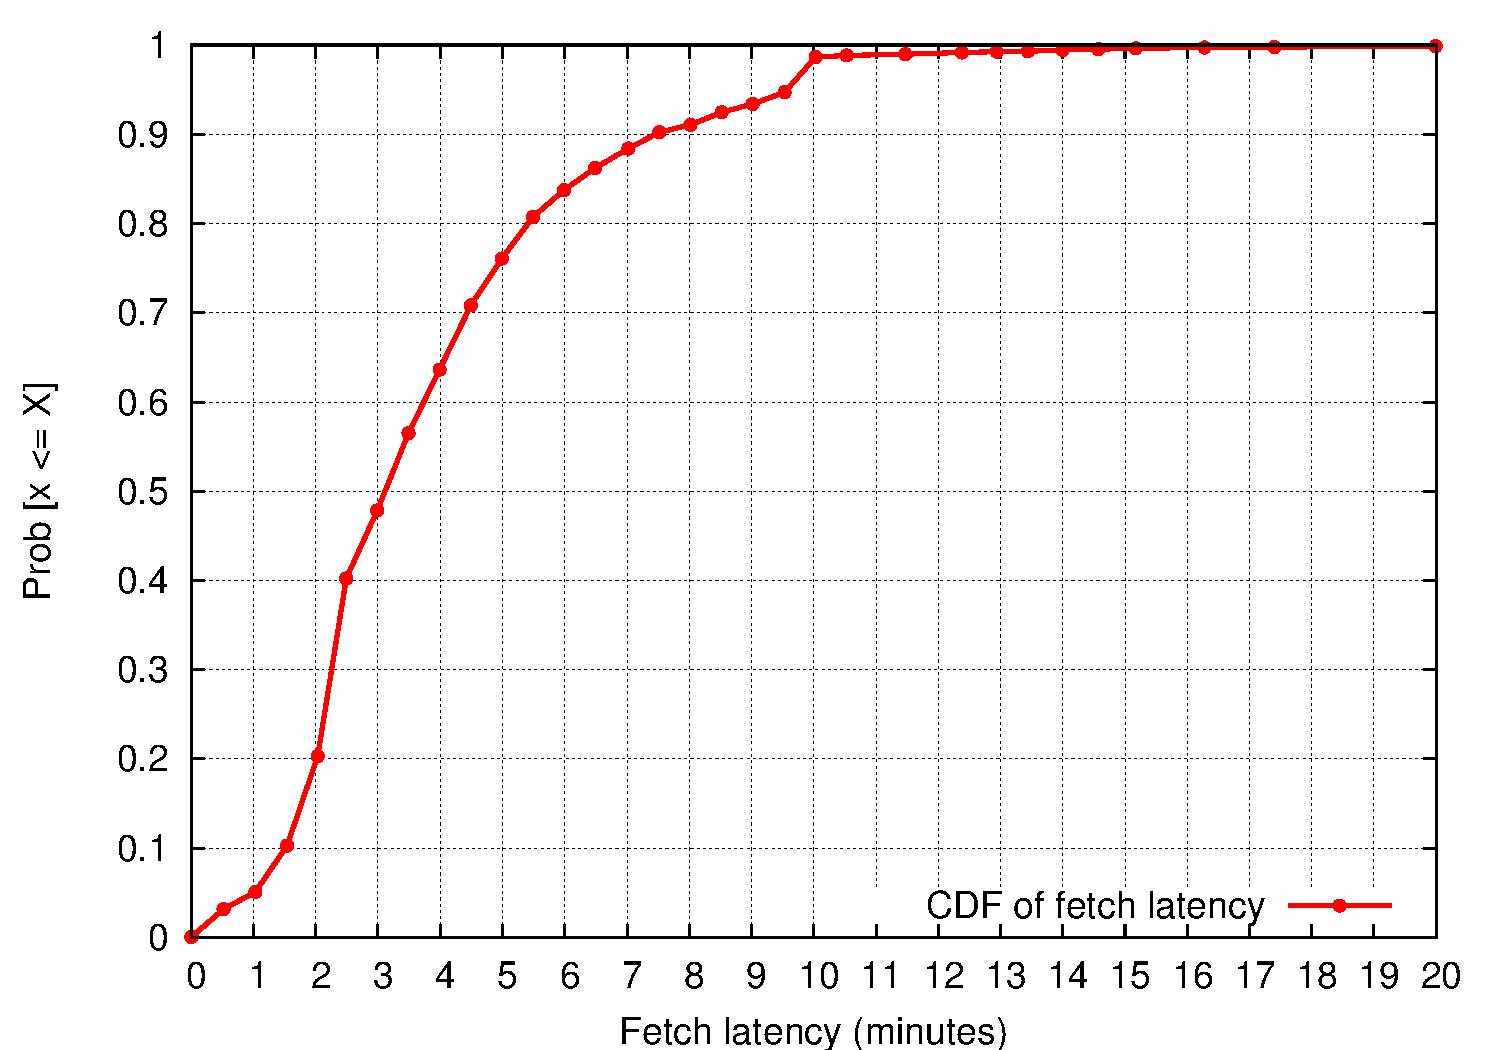
\includegraphics[width=\hsize]{./evaluation/figs/performance/fetchlatency/fetch-latency-cdf.pdf}
%\end{center}
%\caption{\small{\bf Fetch latency.}
%{\em This is a CDF of the latency for each fetch operation on a
%per-node basis. The median latency is just over 3~minutes, and the
%maximum latency (in all but a few cases) is 10~minutes.}}
%\label{fig-fetchlatency}
%\end{figure}

%    - Latency by hopcount
%\begin{figure}[t]
%\begin{center}
%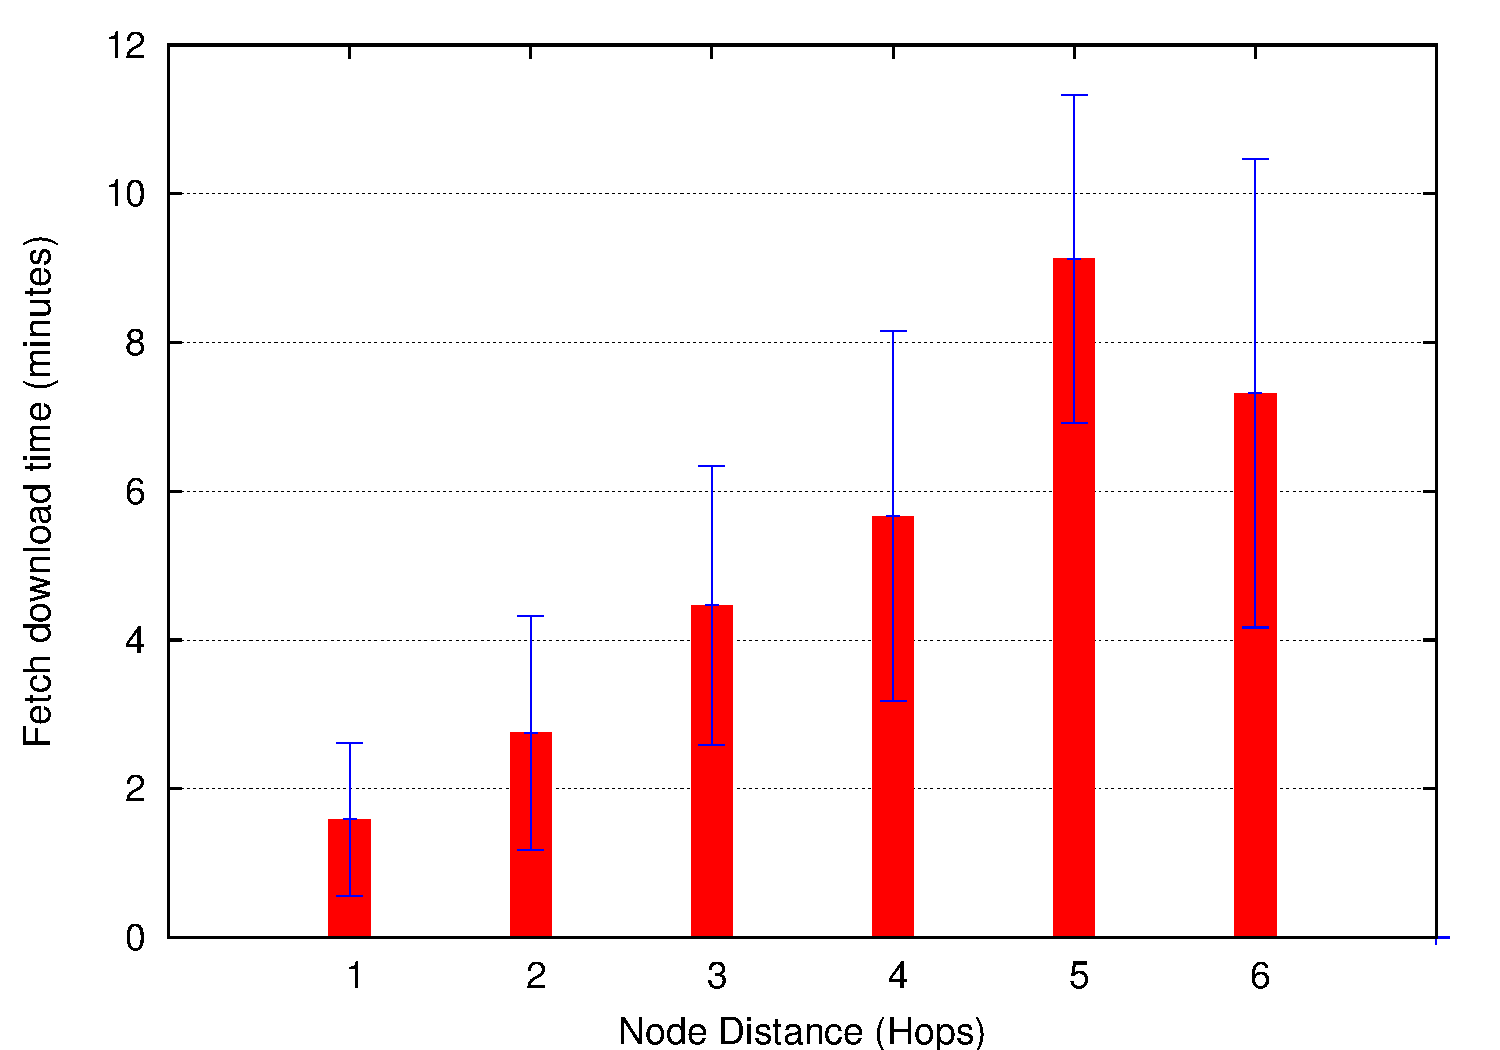
\includegraphics[width=\hsize]{./evaluation/figs/performance/fetchlatency/fetchlatency-byhops.pdf}
%\end{center}
%\caption{\small{\bf Fetch latency by hopcount.}
%{\em The latency for a Fetch download depends on the hop distance of
%the node from the root of the spanning tree, which affects both
%command propagation latency and reliability of the routing path.}}
%\label{fig-fetchlatency-byhops}
%\end{figure}

